\section{Results}
Figure \ref{fig:Searchtimefulltext10} and \ref{fig:Searchtimefulltext11} show the measured search times for the full-text search indices.

\begin{figure}[ht!]
    \centering
    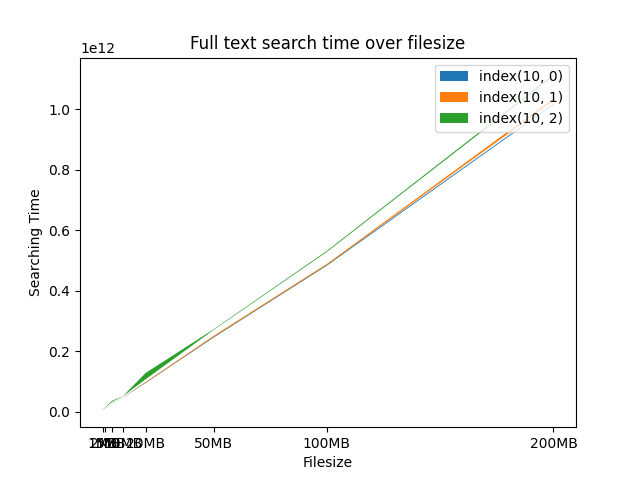
\includegraphics[width=.8\textwidth]{LaTeX/Pictures/Results/Fulltext[(10, 0), (10, 1), (10, 2)].png}
    \caption{Search times for the full-text search function of index 10.0, 10.1 and 10.2. 1000 queries of 5 words. The time on the y-axis is measured in $ns$}
    \label{fig:Searchtimefulltext10}
\end{figure}

\begin{figure}[ht!]
    \centering
    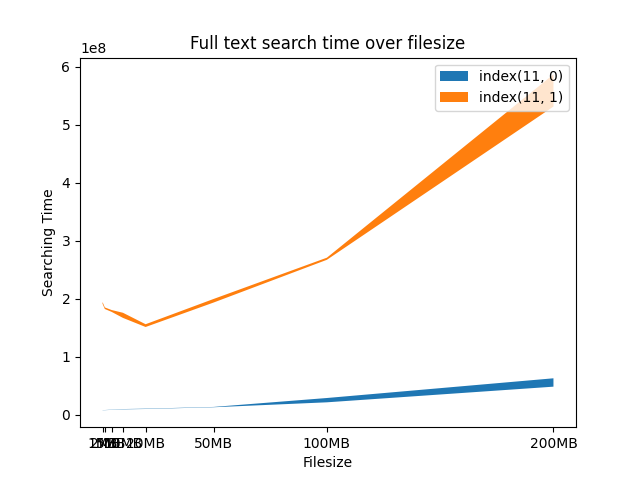
\includegraphics[width=.8\textwidth]{LaTeX/Pictures/Results/Fulltext[(11, 0), (11, 1)].png}
    \caption{Search times for the full-text search function of index 11.0 and 11.1. 1000 queries of 5 words. The time on the y-axis is measured in $ns$}
    \label{fig:Searchtimefulltext11}
\end{figure}

Figure \ref{fig:Searchtimefulltext10long} show the measured search times for the full-text search indices.

\begin{figure}[ht!]
    \centering
    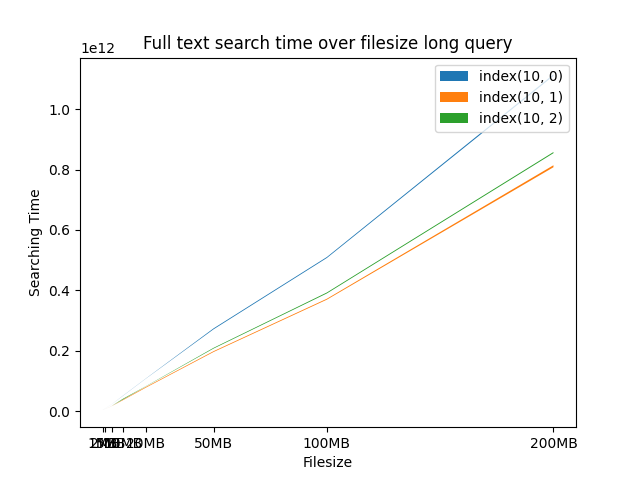
\includegraphics[width=.8\textwidth]{LaTeX/Pictures/Results/Fulltexlong[(10, 0), (10, 1), (10, 2)].png}
    \caption{Search times for the full-text search function of index 10.0, 10.1 and 10.2. 1000 queries of 25 words. The time on the y-axis is measured in $ns$}
    \label{fig:Searchtimefulltext10long}
\end{figure}

Figure \ref{fig:IndexingAll} shows the measured indexing time for the Full text search indices and the Boolean indices for comparison.

\begin{figure}[ht!]
    \centering
    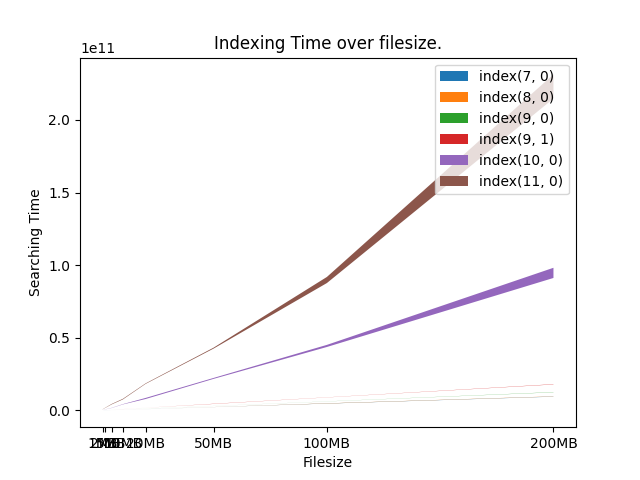
\includegraphics[width=.8\textwidth]{LaTeX/Pictures/Results/Indexing[(7, 0), (8, 0), (9, 0), (9, 1), (10, 0), (11, 0)].png}
    \caption{Indexing times for all indices. The time on the y-axis is measured in $ns$.}
    \label{fig:IndexingAll}
\end{figure}